\documentclass[USenglish]{article}

%\usepackage[utf8]{inputenc}%(only for the pdftex engine)
\RequirePackage[no-math]{fontspec}[2017/03/31]%(only for the luatex or the xetex engine)
\usepackage[small]{dgruyter}

\usepackage{natbib}
\bibliographystyle{apalike}

\usepackage{microtype}

\begin{document}

  \articletype{Research Article}

  \author*[1]{C.J.(Chaojie) Duan}
  %\author[2]{...}
  %\author[1]{...} 
  \runningauthor{Duan}
  \affil[1]{Dulun Consulting Group, research@dulun.com}
  %\affil[2]{...}
  \title{Home Sweet Home Field Advantage:}
  \runningtitle{Bayesian Hierarchical Analysis}
  \subtitle{Examination at Sport, League, and Club Levels}
  \abstract{From 2001 to 2017 seasonal data}
  \keywords{European Professional Soccer Leagues, Home Field Advantage, Poisson generative process}
  %\classification[PACS]{...}
  %\communicated{...}
  %\dedication{...}
  \received{5/21/2018}
  %\accepted{...}
  \journalname{Journal of Quantitative Analysis in Sports}
  %\journalyear{...}
  %\journalvolume{..}
  %\journalissue{..}
  \startpage{1}
  %\aop
  %\DOI{...}
\maketitle

\section{Introduction} 

%The National Football League is tapping Amazon Web Services to help power its “Next Gen Stats” platform.

Aiming to uncover deeper insights into the games of professional football, the National Football League (NFL) recently announced that it will be powering its Next Gen Stats with Amazon's Cloud Computing Platform - AWS to kick off the 2018 season. %with more impactful and meaningful content.  
Amazon’s cloud computing arm also powers Statcast, the next generation statistics platform for Major League Baseball (MLB). These high-profile tech-sport partnerships are arguably the latest and most visible account of invasion of analytics into the realms of spectator sports.

\begin{figure}[ht]
\caption{\textit{Revenue of the top European soccer leagues (Big Five*) from 2006/07 to 2016/17 (in billion euros)}}

\centering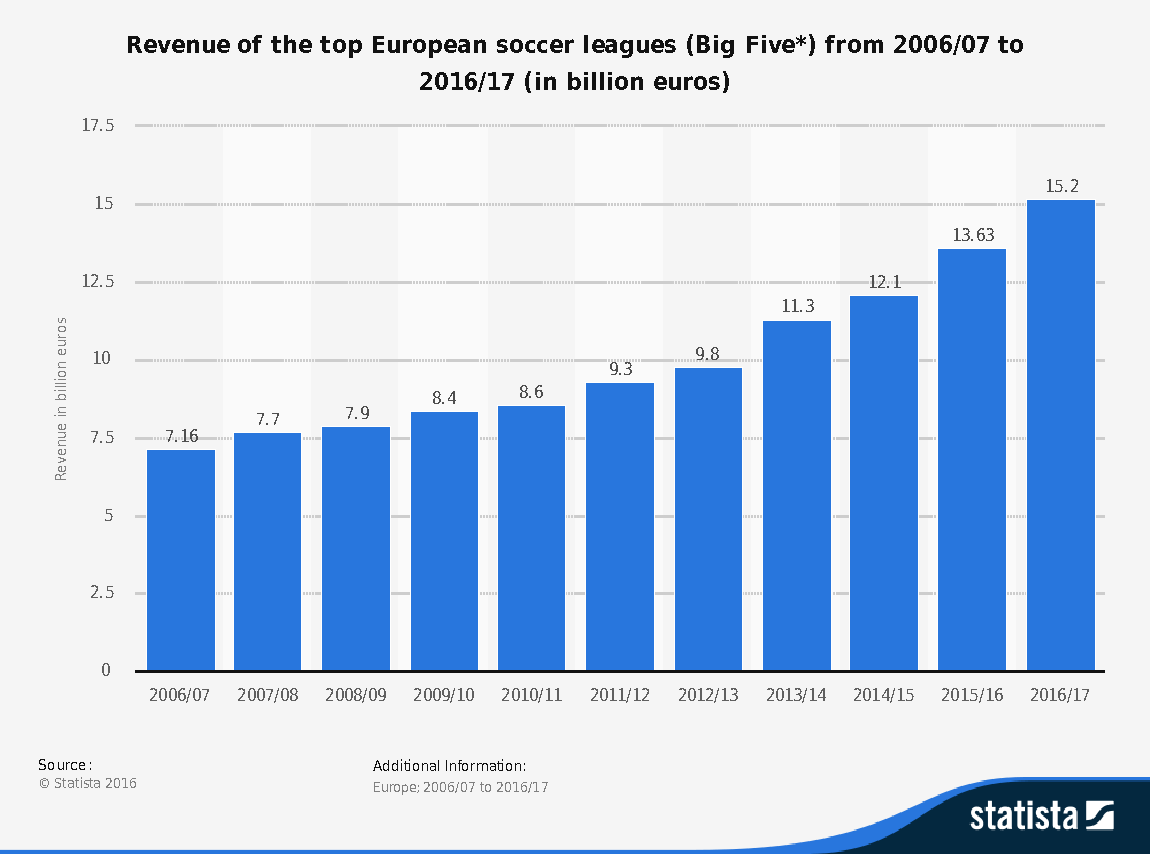
\includegraphics[width=0.8\textwidth]{HFA11.pdf}

\end{figure}


Accompanying the wide-spreading notoriety in the general populace is the ever-increasing availability and volume of data associated with games, players, teams, and sports.   

%a new platform that uses data from player and ball tracking devices to produce new advanced statistics like distance covered, speed, and acceleration — the idea is to better show a receiver’s ability to get open, for example, or how well the offensive line protects the quarterback. The information is shown to fans online and on TV broadcasts; teams also leverage the data internally for strategic purposes.

%we’ll be able to kick off our 2018 season with even more impactful and meaningful content, uncovering deeper insights into the game of football than we’ve ever done before,” 

%Matt Swensson, vice president of emerging products and technology at the NFL, said in a statement. “We chose AWS because of its combination of advanced cloud offering, powerful machine learning capabilities, and experience operating at the scale we need.”





%The popular frequentist (Fisherian) statistical inference process starts with the formulation of an alternative research hypothesis(Ha), such as "people with higher income live happier than low income earners", which is typically set up against a null non-effect hypothesis (Ho), such as ``income level has no effect on happiness". Then researchers collect relevant data (each subject's perceived happiness and income), and conduct a statistical. 

\citep{Gajewski2006}

 


A second motivator for this study is related to the hotly debated topic of home field advantage in soccer competition.
The contributions we made in this paper are (1) highlighting the different generative process underlying most sports performance metrics and suggesting corresponding solutions.  (2) refuting the long and firmly held belief of HFA: (3) contrasting the Bayesian and the frequentist approaches to statistical inference in answering the the same research question and using the same data.
 
\section{Review of Literature} 

%-----------------------
\begin{table}[ht]
\caption{Descriptive Statistics}
\centering
\begin{tabular}{cccccccc}
\starttabularbody
\hline 
 & Mean & Median & Std. Dev. & Min. & Max. & Skewness & Kurtosis\\
\hline
 MHG & 3.634 & 4 & 1.676 & 0 & 9 & 0.246 & 0.034 \\
\hline 
 MAG & 2.884 & 3 & 1.676 & 0 & 10 & 0.627 & 0.786 \\
\hline
\end{tabular}
\label{tab1}
%{Goal Scoring Metrics: Most Home \& Away Goals at the Season Level} 
\end{table}
%=====================================================

\subsection{Data and Analyses} 

 
 

\subsection{Sources} 


\subsection{Results} 


\begin{figure}
\caption{Home Field Advantage Plot at Sport (Professional Soccer) and League Levels}
{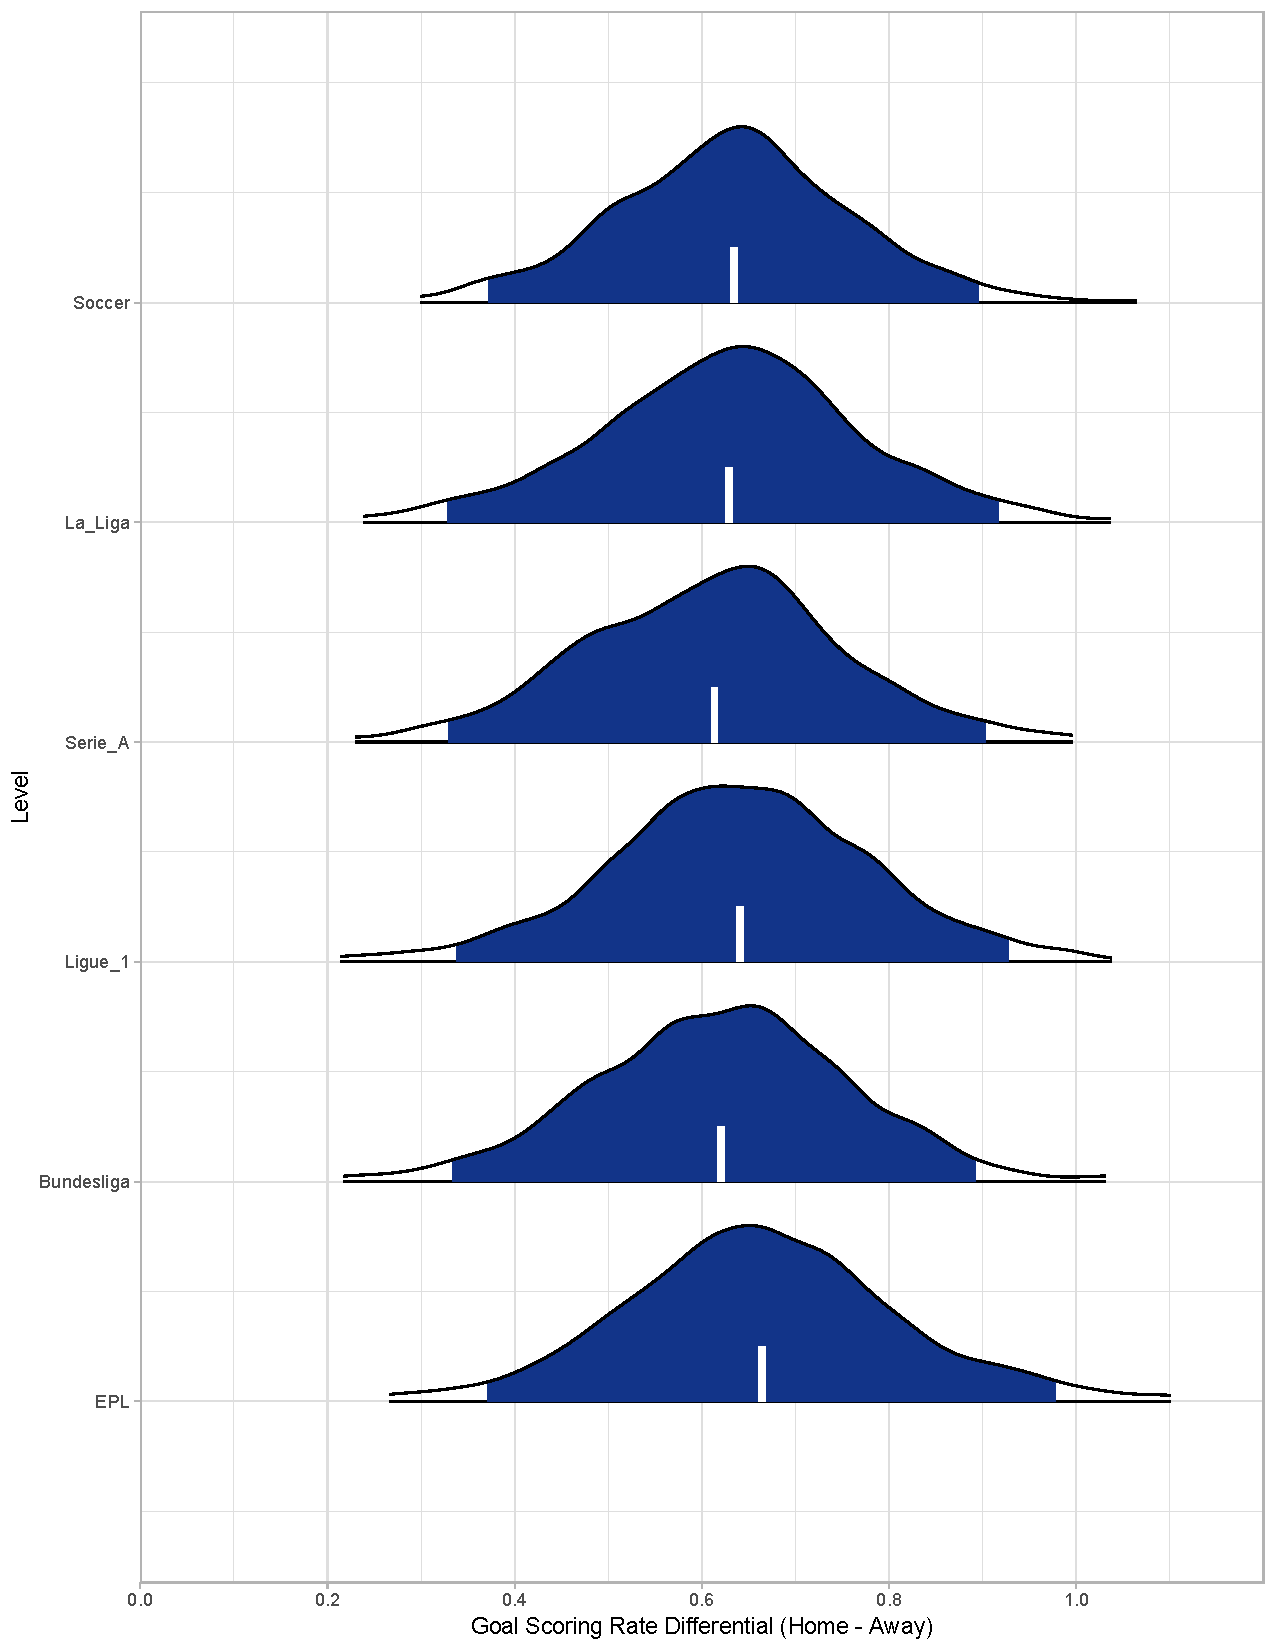
\includegraphics[width=0.80\linewidth]{HFA32.pdf}}
\label{fig1}
\end{figure}

\begin{acknowledgement}

We would like to thank ESPN FC for compiling the season-level club performance data and allow public access.

\end{acknowledgement}

\newpage

%\bibliographystyle{name}
\bibliography{Soccer}
\end{document}
